\documentclass[letterpaper]{article}
\usepackage[margin=1in]{geometry}
\usepackage[utf8]{inputenc}
\usepackage{textcomp}
\usepackage{amssymb}
\usepackage{natbib}
\usepackage{graphicx}
\usepackage{gensymb}
\usepackage{amsthm, amsmath, mathtools}
\usepackage[dvipsnames]{xcolor}
\usepackage{enumerate}
\usepackage{mdframed}
\usepackage[most]{tcolorbox}
\usepackage{csquotes}
% https://tex.stackexchange.com/questions/13506/how-to-continue-the-framed-text-box-on-multiple-pages

\tcbuselibrary{theorems}

\newcommand{\R}{\mathbb{R}}
\newcommand{\Z}{\mathbb{Z}}
\newcommand{\N}{\mathbb{N}}
\newcommand{\Q}{\mathbb{Q}}
\newcommand{\C}{\mathbb{C}}
\newcommand{\code}[1]{\texttt{#1}}
\newcommand{\mdiamond}{$\diamondsuit$}
\newcommand{\PowerSet}{\mathcal{P}}
\newcommand{\Mod}[1]{\ (\mathrm{mod}\ #1)}
\DeclareMathOperator{\lcm}{lcm}

%\newtheorem*{theorem}{Theorem}
%\newtheorem*{definition}{Definition}
%\newtheorem*{corollary}{Corollary}
%\newtheorem*{lemma}{Lemma}
\newtheorem*{proposition}{Proposition}


\newtcbtheorem[number within=section]{theorem}{Theorem}
{colback=green!5,colframe=green!35!black,fonttitle=\bfseries}{th}

\newtcbtheorem[number within=section]{definition}{Definition}
{colback=blue!5,colframe=blue!35!black,fonttitle=\bfseries}{def}

\newtcbtheorem[number within=section]{corollary}{Corollary}
{colback=yellow!5,colframe=yellow!35!black,fonttitle=\bfseries}{cor}

\newtcbtheorem[number within=section]{lemma}{Lemma}
{colback=red!5,colframe=red!35!black,fonttitle=\bfseries}{lem}

\newtcbtheorem[number within=section]{example}{Example}
{colback=white!5,colframe=white!35!black,fonttitle=\bfseries}{def}

\newtcbtheorem[number within=section]{note}{Important Note}{
        enhanced,
        sharp corners,
        attach boxed title to top left={
            xshift=-1mm,
            yshift=-5mm,
            yshifttext=-1mm
        },
        top=1.5em,
        colback=white,
        colframe=black,
        fonttitle=\bfseries,
        boxed title style={
            sharp corners,
            size=small,
            colback=red!75!black,
            colframe=red!75!black,
        } 
    }{impnote}
\usepackage[utf8]{inputenc}
\usepackage[english]{babel}
\usepackage{fancyhdr}
\usepackage[hidelinks]{hyperref}

\pagestyle{fancy}
\fancyhf{}
\rhead{CSE 131}
\chead{Monday, April 10, 2023}
\lhead{Lecture 4}
\rfoot{\thepage}

\setlength{\parindent}{0pt}

\begin{document}

\section{Binary Operations}
We'll now look at adding functionality for binary operations. 

\subsection{Adding Binary Operation Support}
Let's suppose we want to add \code{(+ <expr> <expr>)} to our compiler. Our grammar for our language might look like 
\begin{verbatim}
    (*
        expr := <number> 
            | (add1 <expr>)
            | (sub1 <expr>)
            | (+ <expr> <expr>) 
    *)\end{verbatim}
The \code{Expr} \code{enum} might look like 
\begin{verbatim}
    enum Expr {
        Num(i32),
        Add1(Box<Expr>),
        Sub1(Box<Expr>),
        Plus(Box<Expr>, Box<Expr>),
    }\end{verbatim} 

\subsubsection{Creating the Parser}
Modifying the parser is simple. The \code{parse\_expr} function might look like 
\begin{verbatim}
pub fn parse_expr(s: &Sexp) -> Expr {
    match s {
        Sexp::Atom(I(n)) => Expr::Num(i32::try_from(*n).unwrap()),
        Sexp::List(list) => match &list[..] {
            [Sexp::Atom(S(op)), e] if op == "add1" => 
                Expr::Add1(Box::new(parse_expr(e))),
            [Sexp::Atom(S(op)), e] if op == "sub1" => 
                Expr::Sub1(Box::new(parse_expr(e))),
            [Sexp::Atom(S(op)), e] if op == "negate" => 
                Expr::Negate(Box::new(parse_expr(e))),
            [Sexp::Atom(S(op)), e1, e2] if op == "+" => {
                Expr::Add(Box::new(parse_expr(e1)), Box::new(parse_expr(e2)))
            }
            _ => panic!("parse error"),
        },
        _ => panic!("parse error"),
    }
}\end{verbatim}
Because we know that addition will always be of the form \code{(+ <expr> <expr>)}, we simply need to add a match condition to the inner \code{match} checking if the operation is \code{+}. 

\subsubsection{Modifying the Compiler: Part 1}
Suppose we update the \code{compile\_expr} function so it looks like  
\begin{verbatim}
    fn compile_expr(e: &Expr) -> String {
        match e {
            Expr::Num(n) => format!("mov rax, {}", *n),
            Expr::Add1(subexpr) => compile_expr(subexpr) + "\nadd rax, 1",
            Expr::Sub1(subexpr) => compile_expr(subexpr) + "\nsub rax, 1",
            Expr::Plus(e1, e2) => {
                let e1_instrs = compile_expr(e1);
                let e2_instrs = compile_expr(e2);
                e1_instrs + "\n mov rbx, rax" + &e2_instrs + "\n add rax, rbx"
            }
        }
    }\end{verbatim}

\begin{mdframed}
    (Exercise.) Using the above code for compiling, what is the assembly code generated after compiling the following code? What is the result of running the assembly? 
    \begin{enumerate}[(a)]
        \item \code{(+ (+ 100 30) 4)}
        \begin{mdframed}
            \begin{verbatim}
	mov rax, 500
	mov rbx, rax
	mov rax, 30
	mov rbx, rax
	mov rax, 9
	add rax, rbx
	add rax, rbx
	ret\end{verbatim}
            The result is \code{134}, as expected.
        \end{mdframed}

        \item \code{(+ 500 (+ 30 9))}
        \begin{mdframed}
            \begin{verbatim}
	mov rax, 500
	mov rbx, rax
	mov rax, 30
	mov rbx, rax
	mov rax, 9
	add rax, rbx
	add rax, rbx
	ret\end{verbatim}
            The result is \code{69}, which isn't what we were expecting. Notice how, in the second line, we effectively put \code{500} into \code{rbx}. In the fourth line, we overwrite \code{500} with \code{30}. In any case, this isn't what we were expecting, so option (a) will not work. 
        \end{mdframed}
    \end{enumerate}
\end{mdframed}

\subsubsection{Modifying the Compiler: Part 2}
Clearly, the first attempt at modifying the compiler didn't work. In fact, while this may work for simple addition operations, this won't work for more complex addition operations. 

\bigskip 

One solution is to essentially store important values in the stack, and then refer to the values in the stack when doing addition. This gives us the following code: 
\begin{verbatim}
    fn compile_expr(e: &Expr, si: i32) -> String {
        match e {
            Expr::Num(n) => format!("mov rax, {}", *n),
            Expr::Add1(subexpr) => compile_expr(subexpr, si) + "\nadd rax, 1",
            Expr::Sub1(subexpr) => compile_expr(subexpr, si) + "\nsub rax, 1",
            Expr::Plus(e1, e2) => {
                let e1_instrs = compile_expr(e1, si);
                let e2_instrs = compile_expr(e2, si + 1);
                let stack_offset = si * 8;
                format!("
                    {e1_instrs}
                    mov [rsp - {stack_offset}], rax
                    {e2_instrs}
                    add rax, [rsp - {stack_offset}]
                ")
            }
        }
    }\end{verbatim}
Some technical remarks: 
\begin{itemize}
    \item In our current setting, we do not need to allocate any memory. All we're doing is using is the stack memory, which the operating system gives us. The highest address is where the stack begins, and grows in decreasing address\footnote{All the operating system will do is, if we somehow use the entire stack space, we'll probably end up with a segfault.}. If we need to worry about creating a lot of objects or storing a lot of information on the heap, then we need to allocate memory. 
    
    \bigskip 

    Roughly speaking, this might look like 
    \begin{center}
        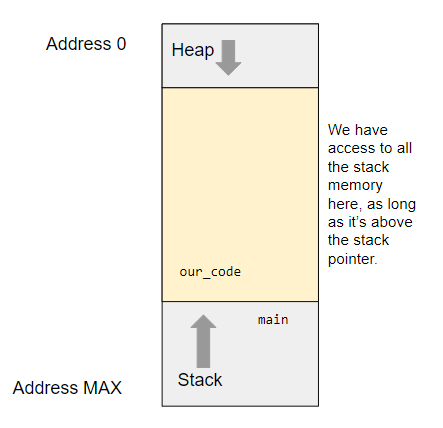
\includegraphics[scale=0.9]{../assets/stack_vis.png}
    \end{center}
    \item \code{rsp} is the register representing the stack pointer. \code{rsp} points to the very bottom of the stack frame that we get to use for all of our generated code. 
    \item In the line \code{si * 8}, the \code{8} represents the size of a Word. This will be \code{8} for a 64-bit machine and \code{4} for a 32-bit machine. 
    \item The \code{si} parameter is the \textbf{stack index}. The stack index should initially be a small positive integer (e.g., 1 or 2). The stack index simply represents how deep in nested expressions or temporary variables we need to save. In this class, we'll prefer using the value \code{2} (i.e., 2 words up from where \code{rsp} is) because the bottom of the stack is where information like the return pointer (how we can use \code{ret}) is stored. We will generally use information one other word at the bottom of the stack.
\end{itemize}
In this sense, we'll initially call \code{compile\_expr} with the arguments \code{e} (our expression to compile) and \code{2} (the stack index).

\begin{mdframed}
    (Exercise.) Using the newly revised code for compiling, what is the assembly code generated after compiling the following code?
    \begin{verbatim}
        (+ (+ 100 50) 2)\end{verbatim}

    \begin{mdframed}
        Roughly speaking, the AST representation of the above code is 
        \begin{verbatim}
Plus(
    Plus(
        Num(100),
        Num(50)
    ),
    Num(2)
)\end{verbatim}

        Drawing out the recursion tree gives us 
        \begin{center}
            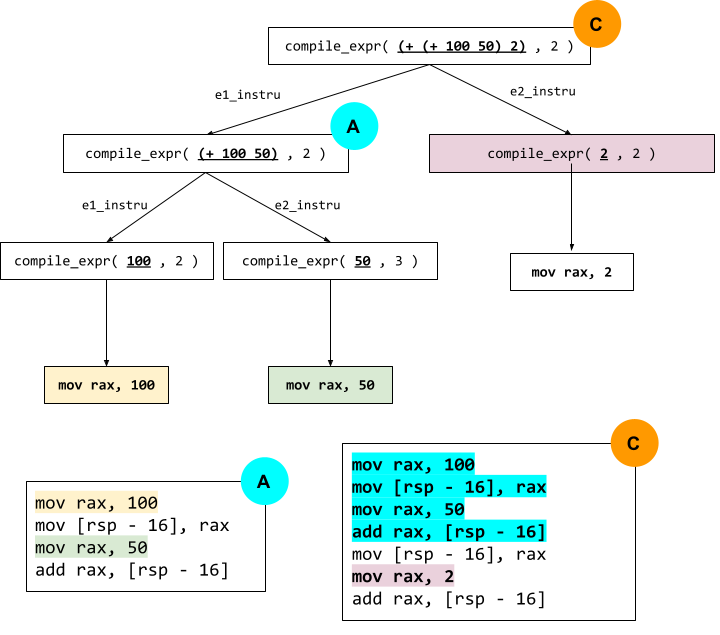
\includegraphics[scale=0.57]{../assets/add_asm.png}
        \end{center}
        Note that the values passed in the function calls are intended to make things more clear, and will not compile otherwise. 
    \end{mdframed}
\end{mdframed}

\bigskip 

Here's the resulting assembly.
\begin{verbatim}
    mov rax, 100
    mov [rsp - 16], rax
    mov rax, 50 
    add rax, [rsp - 16]
    mov [rsp - 16], rax
    mov rax, 2
    add rax, [rsp - 16]\end{verbatim}
Suppose we run through each line of this assembly. This is what the resulting stack memory might look like: 
\begin{center}
    \begin{tabular}{p{2in}|p{4in}}
        Executed Line & Result After Running \\ 
        \hline 
        \code{mov rax, 100} & \raisebox{-\totalheight}{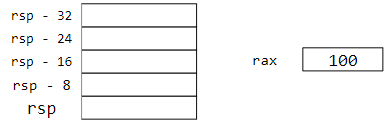
\includegraphics[scale=0.8]{../assets/a1.png}} \\ 
        \hline 
        \code{mov [rsp - 16], rax} & \raisebox{-\totalheight}{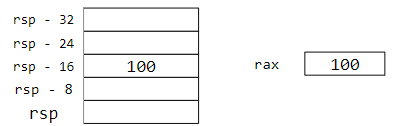
\includegraphics[scale=0.8]{../assets/a2.png}} \\ 
        \hline 
        \code{mov rax, 50} & \raisebox{-\totalheight}{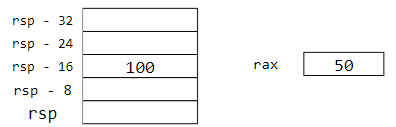
\includegraphics[scale=0.8]{../assets/a3.png}} \\ 
        \hline 
        \code{add rax, [rsp - 16]} & \raisebox{-\totalheight}{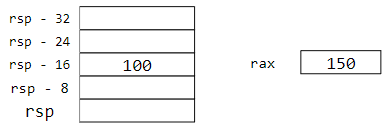
\includegraphics[scale=0.8]{../assets/a4.png}} \\ 
        \hline 
        \code{mov [rsp - 16], rax} & \raisebox{-\totalheight}{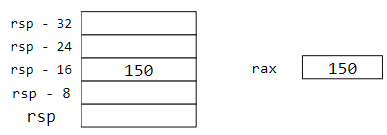
\includegraphics[scale=0.8]{../assets/a5.png}} \\ 
        \hline 
        \code{mov rax, 2} & \raisebox{-\totalheight}{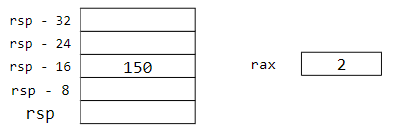
\includegraphics[scale=0.8]{../assets/a6.png}} \\ 
        \hline 
        \code{add rax, [rsp - 16]} & \raisebox{-\totalheight}{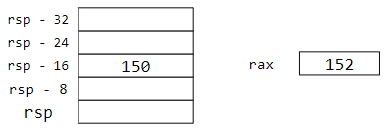
\includegraphics[scale=0.8]{../assets/a7.png}} \\ 
        \hline 
    \end{tabular}
\end{center} 


\end{document}